\section{The Proof-of-Stake Wallet}\label{sec:delegation-transaction}

So far, we have covered the core wallet protocol and functionality and the
respective security analysis. Now, we focus on the wallet's interaction with a
PoS ledger. Specifically, we consider a PoS wallet with access to a core (as
defined by $\FuncW$) and a PoS ledger, which enables a user to issue payments,
participate in the PoS protocol, or delegate stake in the ledger. Specifically,
in this section, we describe how to construct such PoS wallet and describe the
issuing of payments, delegation, stake pool registration, as well as the
generic PoS protocol participation's rules. Finally, we formalize the security
of the ``stake-pooled'' variant of any PoS protocol and describe various modes
of execution of the PoS wallet, which offer enhanced safety and privacy.

Our system depends on the following functions and properties, parameterized by
a chain $\chain$:
\begin{enumerate}
    \item $F_\asset(\cdot)$: given an address $\addr$, the function returns the
        assets that $\addr$ owns;
    \item $F_{\Phi, tx}(\cdot)$: given a transaction $\tx$, the function
        outputs the fees $\Phi$ of publishing $\tx$ on the ledger;
    \item $F_{otx}(\cdot)$: given an address $\addr$, the function outputs the
        number of $\addr$'s outgoing transactions;
    \item $\Phi_{reg}$: the (protocol-specific) cost of stake pool
        registration;
    \item $\addr_{reg}$: a special address that pertains to pool registration;
    \item $F_{PoS, player}()$: given a chain, a function that outputs the next
        participant in the PoS protocol.
\end{enumerate}

\subsection{Payment}\label{subsec:payment}

Payment is the transfer of $\assetset$ assets from a sender's address $\addr_s$
to the receiver's address $\addr_r$. To make a payment, the wallet first
creates an object $\tx = (\assetset, \addr_s, \addr_r, m)$, with some metadata
$m$.  For a UTxO blockchain, the metadata contains a change address $\addr_c$.
For an account-based ledger, the wallet retrieves the number of output
transactions $otx = F_{otx}(\addr_s)$ and adds it to the metadata, as replay
attack protection (see below Section~\ref{sec:stake-pooled-security}). All
addresses are generated via the \emph{Address Generation} interface of
$\FuncW$. Also the wallet calls $F_\asset(\addr_s)$ to retrieve the balance
$\assetset^\prime$ of $\addr_s$ and calculates the fees $\Phi = F_{\phi,
tx}(tx)$.

After ensuring that the address has enough balance, \ie that $(\assetset \cup
\Phi) \subseteq \assetset^\prime$, the wallet sends $(\textsc{Pay}, \tx)$ to
$\FuncW$. When $(\textsc{Transaction}, \tx, \sign)$ is returned, the wallet
publishes it on the network. The signed transaction can be easily verified by
sending $(\textsc{VerifyPay}, \tx, \sign)$ to $\FuncW$ and waiting for the
response $\textsc{VerifiedPay}(\tx, \sign, 1)$.

\subsection{Stake Pool Registration}

A stake pool is identified by a registered staking key. Prior to registration,
the pool's wallet first uses the address generation interface of $\FuncW$ to
compute a staking key $\stakingkeypair$. It then creates a registration
certificate $r = (\stakingkeyverify, m)$, where $m$ is the pool's metadata, \eg
the name of the pool's leader. To register, the wallet sends $(\textsc{Stake},
r)$ to $\FuncW$. Upon receiving $(\textsc{Staked}, r, \sign)$, it publishes
$\Sigma = (r, \sign)$ on the ledger by creating a special payment transaction.
Specifically, the wallet retrieves the registration fees $\Phi_{reg}$ and the
special address $\addr_{reg}$. It then uses an address $\addr_s$, which it
owns, to create  $\tx = (\Phi_{reg}, \addr_s, \addr_{reg}, \Sigma)$, \ie a
transaction including the registration certificate in its metadata. This
transaction is signed and published as above.  To validate a registration
certificate $\Sigma = (r, \sign)$, a party sends $(\textsc{VerifyStake}, r,
\sign)$ to $\FuncW$ and waits for $(\textsc{VerifiedStake}, r, \sign, 1)$.

\subsection{Delegation}\label{subsec:delegation}

Stake delegation is achieved with certificates via a process similar to the
staking pool registration. A delegation certificate is a tuple $d =
(\stakingkeyverify_s, \langle \stakingkeyverify_d, m \rangle )$. The first
element is the staking key $\stakingkeyverify_{s}$, on which the certificate
applies. The second is the staking key $\stakingkeyverify_d$ of the delegate.
The third element is the certificate's metadata. To sign the delegation
certificate, the wallet sends $(\textsc{Stake}, d)$ to $\FuncW$. Upon receiving
$(\textsc{Staked}, d, \sign)$ it publishes $\Sigma = (d, \sign)$ on the ledger,
following the same method as pool registration, \ie via a payment transaction.
As before, a party validates $\Sigma$ via the staking verification interface of
$\FuncW$.

An address with staking object $\beta$ is associated with a staking key
$\stakingkeyverify_s$ in two ways:
\begin{inparaenum}[i)]
    \item \emph{base address}: $\beta = \hash(\stakingkeyverify_s)$;
    \item \emph{pointer address}: $\beta$ needs to point to either a delegation
        certificate $(\stakingkeyverify_s, \cdot, \cdot, \cdot)$ or a
        registration certificate $(\stakingkeyverify_s, \cdot, \cdot)$, \ie the
        pointer address is associated with the staking key defined in the
        certificate to which it points.
\end{inparaenum}

We stress that, when a staking key issues a delegation certificate, \emph{all}
associated addresses are re-delegated accordingly. Specifically, the
certificate to which a pointer address points is used \emph{only} to identify
the staking key with which it is associated, and does not necessarily define
its delegation profile. For example, let $\addr_p$ be a pointer address that
points to delegation certificate $(\stakingkeyverify_s, \stakingkeyverify_d, m,
\sign)$, thus is initially associated with $\stakingkeyverify_s$. Now,
$\stakingkeyverify_s$ publishes a newer certificate $(\stakingkeyverify_s,
\stakingkeyverify_d', m', \sign')$. All addresses associated with
$\stakingkeyverify_s$, including $\addr_p$, are now delegated to
$\stakingkeyverify_d'$. Figure~\ref{fig:delegation} illustrates delegation for
various types of addresses.

\begin{figure}
    \begin{center}
      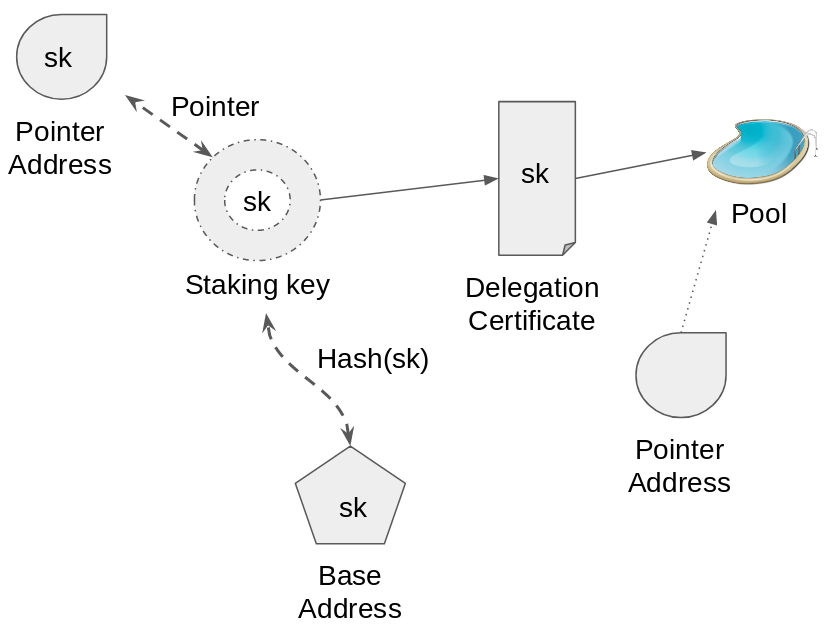
\includegraphics[width=0.6\columnwidth]{figures/delegation/delegation.png}
    \end{center}
    \caption{
        A representation of the delegation mechanism. Base pointers are linked
        to a key via a hash, whereas pointers may point to either a staking key
        or a pool directly.
    }
    \label{fig:delegation}
\end{figure}

Delegation certificates come in two forms, depending on how they are published.
\emph{Heavyweight} certificates are published on the ledger and are identified
by an \emph{index}, which represents the position of the certificate in the
ledger. The index is the tuple $ptr = (b, x, c)$, where $b$ relates to a block
in the ledger, $x$ represents a transaction in $b$, and $c$ identifies a
certificate in the metadata of $x$. Therefore, every pointer address contains
the index of the certificate to which it points. If an address $\addr$ points
to an invalid certificate, then $\addr$'s stake is not delegated.
\emph{Lightweight} certificates are not published by default, but instead
become public when their staking key participates in the PoS protocol.
Conflicts are resolved based on seniority. For instance, let $\stakingkeypair$
be a staking key which issues two certificates $\Sigma_1, \Sigma_2$. If they
are published on the ledger in that order, $\Sigma_2$ takes effect for all
addresses associated with $\stakingkeypair$. The metadata of a lightweight
certificate also contain a ``counter'', \ie an integer that breaks ties between
lightweight certificates; if two conflicting lightweight certificates are
presented, then whichever has the higher counter is accepted.

\paragraph{Certificate length}\label{sec:certificate-evaluation}
Let the curve of the ECDSA scheme be
\emph{secp256r1}~\cite{gupta2004ecc} and the hash function be \emph{SHA256}.
The staking pool registration certificate is the tuple $\Sigma =
(\stakingkeyverify, m, \sign)$. The public key size for $\stakingkeyverify$ (in
the compressed form) is $33$ bytes and the signature $\sign$ is $132$ bytes.
The metadata value $m$ depends on the implementation; for simplicity, we can
assume that it consists of only a hash, so its length is $32$ bytes. Therefore,
the staking pool certificate is $197$ bytes. The delegation certificate is the
tuple $\Sigma = (\stakingkeyverify_s, \stakingkeyverify_{delegate}, m, \sign)$.
As before, the public keys $\stakingkeyverify_s, \stakingkeyverify_{delegate}$
are $33$ bytes each, whereas the signature $\sign$ is $132$ bytes. The metadata
$m$ contains the counter for the lightweight certificates; setting it to $1$
byte enables up to $256$ conflicting lightweight certificates. Therefore,
heavyweight and lightweight delegation certificates are $198$ and $199$ bytes
respectively.

\subsection{Protocol Participation}\label{sec:protocol-participation}

Participation in the PoS protocol consists of publishing specially-crafted,
protocol-related, signed messages. The address which is responsible for
participation at any given time is decided by the function $F_{PoS,player}$ and
its staking key is used to sign these messages. Here, we consider the typical
example of PoS participation, \emph{block generation}, \ie the act of extending
an existing chain with a newly-created block. For simplicity, a block is a
tuple $(\stakingkeyverify, m)$, where $\stakingkeypair$ is the staking key
which issues the block and $m$ is the block's contents, \ie the headers, the
tree of transactions, etc. As with delegation and stake pool registration, the
wallet obtains a signature for a new block via the staking interface of
$\FuncW$, while a verifier can similarly check it. However, whether a block is
valid for a given ledger, \ie whether a block can extend a chain, depends on
the protocol's chain validity rules. Notably, delegation affects these rules.
Next, we describe the validity rules in the presence of delegation, as well as
the rules that pertain to chain delegation, \ie the re-delegation of delegated
stake.

\paragraph{Block Validity}
For a chain $\chain$, the chosen address $\addr_{PoS}$ is associated with a
staking key $\stakingkeyverify_{PoS}$ and a candidate block $\block$ is signed
by a different staking key $\stakingkeypair$. The rules for deciding if
$\block$ is valid for $\chain$ are as follows:
\begin{itemize}
    \item if a delegation certificate for $\stakingkeyverify$ is published in
        $\chain$, $\block$ is invalid;
    \item else if a certificate that delegates from $\stakingkeyverify_{PoS}$
        to $\stakingkeyverify$ is published in $\chain$, $\block$ is valid;
    \item else if either no delegation for $\stakingkeyverify_{PoS}$ or a
        certificate that delegates from $\stakingkeyverify_{PoS}$ to
        $\stakingkeyverify_h$ is published in $\chain$ and $\block$ contains a
        lightweight certificate delegating from $\stakingkeyverify_h$ to
        $\stakingkeyverify$, $\block$ is valid;
    \item else $\block$ is invalid.
\end{itemize}

\paragraph{Chain Validity}
The empty chain $\chain = \epsilon$ is valid. Given a candidate chain $\chain =
\chain' || \block$, if $\chain'$ is valid and the block $\block$ is valid for
$\block$, then $\chain$ is valid.

\paragraph{Chain Decision}
Assume $\chain$ is the chain stored locally by the wallet and $\mathbb{C}$ is
the set of valid chains available on the network. The longest valid chain from
$\mathbb{C} \cup \{ \chain \}$ is chosen. In case of tie between two valid
chains $\chain_1$ and $\chain_2$, where $\head(\chain_1)$ and $\head(\chain_2)$
are signed by $(\stakingkeyverify_1, \stakingkeysign_1)$ and
$(\stakingkeyverify_2, \stakingkeysign_2)$ respectively, the following rules
apply:
\begin{itemize}
    \item if $\stakingkeyverify_1$ and $\stakingkeyverify_2$ are delegated via
        the heavyweight certificates $\Sigma_1$ and $\Sigma_2$, with indexes
        $idx_1$ and $idx_2$ respectively, $\chain_1$ is chosen if $idx_1 >
        idx_2$, otherwise $\chain_2$ is chosen;
    \item else if $\stakingkeyverify_1$ is delegated via the heavyweight
        certificate $\Sigma_1$ and $\stakingkeyverify_2$ is delegated via the
        \emph{lightweight} certificate $\Sigma_2$, $\chain_1$ is chosen;
    \item else if $\stakingkeyverify_1$ and $\stakingkeyverify_2$ are delegated
        via a combination of heavyweight and lightweight certificates
        $(\Sigma_{1,1}, \Sigma_{1,2})$ and $(\Sigma_{2,1}, \Sigma_{2,2})$
        respectively, then:
        \begin{itemize}
            \item if $\Sigma_{1,1}$ and $\Sigma_{2,1}$ have different indexes,
                then choose the one with the higher index;
            \item else if $\Sigma_{1,2}$ and $\Sigma_{2,2}$ have different
                counters, then choose the one with the higher counter;
            \item else choose the first observed on the network.
        \end{itemize}
\end{itemize}

\paragraph{Delegation Chains}\label{sec:chain_delegation}
Chain delegation is the ability of a staking key to re-delegate stake that has
been delegated to it. As described in Section~\ref{subsec:delegation}, the
metadata section of a delegation certificate defines the rules that pertain to
the certificate. One such rule relates to chain delegation. The metadata entry
for this property is a boolean value, ``allowChain'', which identifies whether
chain delegation is allowed for the applicable stake of the certificate.  For
example, let two certificates $\Sigma_0$ and  $\Sigma_1$, where $\Sigma_0$
delegates from a key $\stakingkeyverify_0$ to $\stakingkeyverify_2$ and sets
$\text{``allowChain''} = true$, whereas $\Sigma_1$ delegates from
$\stakingkeyverify_1$ to (the same key as before) $\stakingkeyverify_2$ and
sets $\text{``allowChain''} = false$. Suppose now that a third certificate
$\Sigma_3$ is published, delegating from $\stakingkeyverify_2$ to
$\stakingkeyverify_3$.  Although $\stakingkeyverify_3$ is eligible to
participate on behalf all addresses associated with $\stakingkeyverify_0$, it
cannot participate for those associated with $\stakingkeyverify_1$, since the
corresponding key is $\stakingkeyverify_2$ (as chain delegation is not
permitted for this key).  More concretely, a delegation chain is a list of
certificates $[\Sigma_1, \ldots, \Sigma_i]$ such that, for each certificate
$\Sigma_j, 1 < j \leq i$, it holds that $\Sigma_{j-1}[\stakingkeyverify_{d}] =
\Sigma_j[\stakingkeyverify_s]$  We say that $\stakingkeyverify$ is delegated
via a hain $[\Sigma_1, \ldots, \Sigma]$ if $\Sigma[\stakingkeyverify_{d}] =
\stakingkeyverify$.

\subsection{Security in the Presence of Stake Pools}\label{sec:stake-pooled-security}

In this section, first we analyze the security of stake pools \wrt the
underlying PoS protocol's security assumptions (cf.
Corollary~\ref{cor:stake-pooled}). Next, we discuss prominent hazards, namely
\emph{sybil} and \emph{replay} attacks.

\paragraph{Stake-pooled Security}
The security analysis of a PoS stake-pooled variant, \ie a PoS protocol with
stake pools, is based on the protocol's honest stake threshold assumption
$\tau$. This parameter identifies the minimum percentage of honest stake needed
for the protocol to be secure. It is typically set to $\frac{1}{2} + \epsilon$
or $\frac{2}{3} + \epsilon$, for some $\epsilon > 0$. For simplicity, we assume
that all stake is delegated to a total number of $P$ pools. Each pool possibly
controls a different amount of stake.  Let $P_h$ be the honest pools among $P$,
which control an aggregate $\rho_h$ percentage of the total stake.  When a
player delegates their stake, they effectively relinquish their staking rights.
Therefore, as Corollary~\ref{cor:stake-pooled} shows, the focus should be put
on the adversarial power over pools, rather than stake itself.  For example, if
the adversary delegates some stake to an honest pool, then this stake becomes
honest in the stake-pooled setting, as it is controlled by an honest leader.
Intuitively, the adversary compromises the stake-pooled variant's security by
corrupting an appropriate amount of pools, such that honestly-controlled stake
percentage is less than $\tau$. We stress that this does not imply that the
adversary is required to corrupt a large number of pools. For instance, if a
single pool controls $\rho_a \geq 1-\tau$ of the total stake, then the
adversary can compromise security by only corrupting this single, albeit large,
pool.

\begin{corollary}\label{cor:stake-pooled}
    The stake-pooled variant of a PoS protocol $\pi$ is secure if $\rho_h \geq
    \tau$, where $\rho_h$ is the percentage of the total stake controlled by
    pools which are managed by honest leaders and $\tau$ is the honest stake
    threshold assumption of $\pi$.
\end{corollary}

\paragraph{Sybil Attacks}
Using stake pools for the PoS protocol's execution, rather than the
stakeholders themselves, introduces the possibility of \emph{sybil
attacks}~\cite{douceur2002sybil}. Specifically, suppose that the adversary
creates a large number of stake pools. Honest players cannot immediately
identify whether a pool is adversarial, so these pools could appear legitimate
and (honest) users might be convinced to delegate to them, thus increasing the
adversarial stake ratio. This is an inherent problem to decentralized PoS
systems, as no form of external identification exists and an adversary can
easily create a large number of staking keys and registration certificates. A
potential countermeasure is to have pool leaders commit (some of) their own
stake to their pool.  In our setting, this method can be facilitated via an
extra field in the delegation certificate's metadata, which identifies the
leader's addresses and funds, which are committed to the pool. Evidently, as
long as these funds are locked in the corresponding addresses, a malicious
leader cannot use them for multiple pool commitments. While this does not
directly prevent a Sybil attack, it does force the attacker to commit some
stake to its pools, hence bounding its identity production capabilities.

\paragraph{Replay Attacks}
Another important consideration is replay protection. Replay attacks are
prominent in account-based ledgers, where an adversary may re-publish past
transaction. For instance, suppose Alice sends $x$ assets from her
address-account $\addr$ to Bob. After the payment is published, $\addr$
controls $y = z - x$ assets, $z$ being the funds that $\addr$ controlled before
Alice made the payment. In a replay scenario, Bob re-publishes this payment,
such that a further amount $x$ of funds is sent from Alice's account $\addr$ to
Bob's. The same vulnerability exists against the certificates of our scheme.
For instance, an attacker can re-publish a certificate to forcefully change a
user's delegation choice. To solve this issue, we employ an address
\emph{whitelist}. Specifically, each certificate defines the addresses allowed
to publish it. Naturally, this scheme assumes that the wallet knows these
addresses a priori.  Next, during certificate verification, a party checks
whether it is published in a transaction issued by a whitelisted address.  To
replay the certificate, the adversary would then need to obtain the private
payment key of one of the whitelisted addresses. Notably, our solution requires
no state to be maintained by the verifiers, as the information needed to
counter a replay attack, \ie the address whitelist, exists in the certificate
itself. Therefore, there is no the need to parse the entire ledger or maintain
extra local state, as is the case with counter-based replay protection
mechanisms~\cite{ethereumReplay}.
